\documentclass[10.5pt]{article}
\usepackage{amsfonts, amsmath, amssymb}
\usepackage{multirow, multicol}
\usepackage{epsfig, subfigure, subfloat, graphicx}
\usepackage{anysize, indentfirst, setspace}
\usepackage{verbatim, rotating, paralist}
\usepackage{caption, hanging}
\usepackage{pstricks, sgamevar, egameps}
\usepackage{tikz}
\usepackage{hyperref}
\usetikzlibrary{shapes,arrows,backgrounds,decorations.pathmorphing,decorations.pathreplacing}
% These are the key packages.  There is also sgame instead of sgamevar, but it doesn't work with beamer or other macros.
% The dcolumn package interferes with these, so you need to remove it from your preamble.

\newcommand{\mc}[1]{\multicolumn{1}{c}{#1}}
% I believe this is a command that the package wants to use, though not sure what it's doing and this document seems to compile ok without it, so who knows.


% Note: If you include any extensive form games, you need to compile it in the special 3-step way (in WinEDT): LaTeX, dvi->ps, ps->pdf.

\title{Drawing Games and Diagrams in \LaTeX}
\author{Dave Ohls \\ University of Wisconsin \\ ohls@wisc.edu}
\date{}

\begin{document}



\maketitle

This document introduces a number of ways to draw game matrices, decision and interaction trees, spatial models, and other diagrammatic representations of aspects of strategic behavior.  The code can look a bit dense and intimidating at first, but once you get familiar with what each command (and each part of each command) is doing, these packages provide very flexible ways to draw just about any diagram you want.   \\



\end{document} 


\section{Strategic Form Games}

To make strategic form games, the `game' environment (using the .sgamevar package) behaves much like tabular environments (in fact, you could just use tables instead if you're sophisticated in how you manage the lines).  But using this package does incorporate a few nice features: it automatically places lines in the appropriate places, it does the alignment and dimensions for you, and it centers the player and name labels horizontally and vertically.  Syntactically, it behaves exactly like the tabular environment except:\\

\begin{compactitem}
\item You use the `figure' float instead of the `table' float.
\item The \verb+\>+ replaces \verb+&+ as the divider between cells. %Note: in the sgame package, you use & still
\item The initial operators are different - rather than \verb+\begin{tabular}{l|cc}...\end{tabular}+ it is: \\ \verb+\begin{game}{rows}{columns}[player 1 label][player 2 label][figure label]...\end{game}+ \\
\end{compactitem}


\begin{figure}[h!]
\begin{center}
\begin{footnotesize}
\begin{game}{2}{3}[1][2][]
        \> Left \> Center \> Right   \\
Up      \> 3,2  \> 4,4    \> 5,1   \\
Down    \> 0,0  \> 2,6    \> 4, 3 \\
\end{game}
\end{footnotesize}
\end{center}
\end{figure}


\begin{figure}[h]
\begin{center}
\begin{scriptsize}
\begin{game}{7}{7}[\textbf{US}][\textbf{USSR}][If you like, strategic games can be quite large]
          \> Retreat  \>  Negotiate  \> Sanctions    \> Blockade   \> Airstrike  \> Invade  \> Nuclear\\
Retreat   \> 2,2      \>  2,6        \> 1,5          \> 4,3        \> 2,3        \> 3,4     \> 3,7  \\
Negotiate \> 6,2      \>  8,8        \> 3,5          \> 3,2        \> 1,1        \> 4,0     \> 2,4  \\
Sanctions \> 5,1      \>  5,3        \> 2,2          \> 2,4        \> 0,4        \> 2,5     \> 0,1  \\
Blockade  \> 3,4      \>  2,3        \> 4,2          \> 2,2        \> 7,6        \> 4,7     \> 0,1  \\
Airstrike \> 3,2      \>  1,1        \> 4,0          \> 6,7        \> 4,4        \> 5,5     \> 0,1  \\
Invade    \> 4,3      \>  0,4        \> 5,2          \> 7,4        \> 5,5        \> 6,6     \> 0,3  \\
Nuclear   \> 7,3      \>  4,2        \> 1,0          \> 1,0        \> 1,0        \> 3,0     \> -5,-5 \\
\end{game}
\end{scriptsize}
\end{center}
\end{figure}

\clearpage

You can cluster multiple strategic games together by including them within the same `figure' float, or by having them clustered.  Here, I used the \verb+\hspace{}+ and \verb+\vspace{}+ commands to have them spaced how I wanted.


\begin{figure}[h!]
\begin{center}
\begin{footnotesize}
\begin{game}{2}{2}[1][2][(a)]
        \> Polisci \> Econ \\
Polisci \> 4,4     \> 2,1  \\
Econ    \> 1,2     \> 3,3  \\
\end{game}\hspace{.5in}
\begin{game}{2}{2}[1][2][(c)]
             \> IR   \> Theory   \\
Comparative  \> 5,6  \> 3,3      \\
American     \> 2,3  \> 4,0      \\
\end{game}
\end{footnotesize}
\end{center}
\end{figure}
\vspace{-.3in}
\begin{figure}[h!]
\begin{center}
\begin{footnotesize}
\begin{game}{2}{2}[1][2][(b)]
        \> Dayton \> Mifflin \\
Gorham  \> -4,-2  \> -2,-5   \\
Johnson \> -1,-4  \> -3,-1   \\
\end{game}\hspace{.5in}
\begin{game}{2}{2}[1][2][(d)]
             \> Nash \> Harsanyi \\
von Neumann  \> 1,2  \> 4,3      \\
Morganstern  \> 5,7  \> 0,4      \\
\end{game}
\end{footnotesize}
\end{center}
\end{figure}




\section{Extensive Form Games}
% NOTE: To Texify documents with extensive form games, you must now use a 3-step compiling approach: first click on "LaTeX", then on "dvi->ps", then on "ps->pdf"
% NOTE: For this section, you will need Ghostscript installed.  If you don't have it, go to http://pages.cs.wisc.edu/~ghost/gsview/, click on 'Ghostscript', download the appropriate exe file (at the bottom of the page) and install it.  Then check that the execution mode is correct.

The `egame' environment (in the .egameps package) allows you to draw extensive form games with all sorts of cool features.  Essentially, you define a box, and then draw your game tree by specifying where you want objects (mostly lines) to start, what angle they have, how long they are, how many of them there are, how they are labeled, etc.  A simple version of this looks like: \\



\begin{figure}[h]
\begin{footnotesize}
\begin{center}
\begin{egame}(700,300)
\putbranch(350,250)(3,1){300} \iib{p}{1}{2}[a][b]
\end{egame}
\end{center}
\end{footnotesize}
\end{figure}

%NOTE: it can be very easy to accidently use parenthesis where you should have curly brackets, or vice versa.  If you're getting syntax errors, that's often the problem - move your cursor through the table and see if red pops up anywhere, or comment-out one branch at a time.

What the commands are doing: \\

\begin{compactitem}
\item \verb+\begin{egame}(700,300)... \end{egame}+: Creates an extensive game environment with a box of dimensions 700 horizontally by 300 vertically.
\item \verb+\putbranch(350,250)...+: Begins a branch at location 350 horizontally, 250 vertically (middle of the box, near the top).
\item \verb+...(3,1)...+: Specifies that for each 3 units horizontally, the line should move down 1 unit vertically.
\item \verb+...{300}...+: Specifies that the lines should cover 300 units in the horizontal dimension
\item \verb+...\iib{p}{1}{2}[a][b]+: Specifies 2 (ii) branches, player name p, action label 1 and payoff a on the left branch and action label 2 and payoff b on the right branch. \\
\end{compactitem}

\clearpage

To add in additional components that connect to these, figure out where your branches end up and start new branches there.  Since the initial branches began at (350,250), went over 300 units, and went down 100 units (1 unit down for every 3 units over), they should end at (50,150) and (650, 150).  Lets put a branch in at the end of one of those nodes:
\begin{verbatim}
\putbranch(650,150)(2,1){200} \iiib{other}{$\alpha$}{$\beta$}{$\gamma$}[x,x][y,y][z,z]
\end{verbatim}


\begin{figure}[h]
\begin{footnotesize}
\begin{center}
\begin{egame}(700,300)
\putbranch(350,250)(3,1){300} \iib{player name}{action 1}{action 2}[payoff a][]
\putbranch(650,150)(2,1){200} \iiib{other}{$\alpha$}{$\beta$}{$\gamma$}[x,x][y,y][z,z]
\end{egame}
\end{center}
\end{footnotesize}
\end{figure}

% (I removed the payoff b above, since that is no longer a terminal node)
% In theory, you want to stay within the bounds of your box.  In practice, that's not strictly necessary - you'll notice I have a node starting at 650 and going over 200 (to 850), whereas my box only goes to 700.  Usually that won't be a problem if you're a bit over (or under, in negative numbers), but in some cases it may cause your figure to run off the side of the page or run into other material above or below it.


Now lets do something a bit more complicated.  The figure below uses mostly the same commands that have already been introduced, but expands them to a larger and more interesting game.  It also introduces the information set command, which puts in a horizontal info set starting at the coordinates specified of the length specified, and with a label (if you include one):
\begin{verbatim}
\infoset(200,400){600}{\textbf{Soviet Union}}
\end{verbatim}

\begin{figure}[h]
\begin{footnotesize}
\begin{center}
\begin{egame}(1000,550)
\putbranch(500,500)(3,1){300} \iib{\textbf{Nature}}{Strong NATO ($p$)}{Weak NATO ($1-p$)}
\infoset(200,400){600}{\textbf{Soviet Union}}
\putbranch(200,400)(2,1){200} \iib{}{A}{N}[][0,0,0]
\putbranch(800,400)(2,1){200} \iib{}{A}{N}[][0,0,0]
\putbranch(0,300)(1,1){100} \iib{\textbf{Europe}}{BD}{R}[10,-4,0][]
\putbranch(600,300)(1,1){100} \iib{\textbf{Europe}}{BD}{R}[10,-4,0][]
\putbranch(100,200)(1,1){100} \iib{\textbf{U.S.}}{SO}{I}[5,-8,-8][-5,-2,-2]
\putbranch(700,200)(1,1){100} \iib{\textbf{U.S.}}{SO}{I}[5,-8,0][-5,-2,-2]
\end{egame}
\end{center}
\end{footnotesize}
\end{figure}

\vspace{-.5cm}

The default setting for extensive form games is to set them up vertically (as these have been) but you may also have some you'd rather do horizontally.  To do that, add \verb+\egdirection{r}+ after beginning the egame environment, and all subsequent commands will operate horizontally, moving to the right instead of down (you can also put `l' or `u' for left or up).

\begin{figure}[h]
\begin{footnotesize}
\begin{center}
\begin{egame}(900, 500)
\egdirection{r}
\putbranch(100, 250)(1,1){150}\iib{1}{U}{D}[][]
\putbranch(250, 400)(2,1){200}\iib{2}{l}{r}[4,1][]
\putbranch(250, 100)(2,1){200}\iib{2}{l}{r}[0,0][3,5]
\putbranch(450, 300)(3,1){300}\iib{1}{u}{d}[6,5][8,-4]
\end{egame}
\end{center}
\end{footnotesize}
\end{figure}

\clearpage

Putting all these together, you can do some fancier things like signaling games, bargaining games, or other game structures.  To do the ones below, a few more commands are introduced: \\

\begin{compactitem}
\item \verb+\putbranch(50,250)(2,1)[l]...+: This overrides the `right' orientation of the game as a whole, saying that this particular branch should have a left orientation.
\item \verb+\egalhshift=30+: This introduces a horizontal shift in the action labels.  If your labels are running into each other, or not showing up where you want, you can mess around with this a bit.
\item \verb+\iib{City}[u]...+: This places the player label up from the node (you can also put `d', `l', `r', or `o' for down, left, right, or over the node).
\item \verb+\iib[linecolor=green]+: Makes the lines of those branches green.\\
\end{compactitem}

\vspace{.5cm}

\begin{figure}[h]
\begin{footnotesize}
\begin{center}
\begin{egame}(800,300)
\egdirection{r}
\putbranch(400,150)(0,1){100} \iib{\textbf{N}}{Brutal (.5)}{Soft (.5)}
\putbranch(400,250)(1,0){350} \ib{\textbf{Khan}}[u]{Burn}
\putbranch(400,250)(1,0)[l]{350} \ib{\textbf{}}{Negotiate}
\putbranch(400,50)(1,0){350} \ib{\textbf{Khan}}[d]{Burn}
\putbranch(400,50)(1,0)[l]{350} \ib{\textbf{}}{Negotiate}
\putbranch(750,250)(2,1){150} \egalhshift=30 \iib{\textbf{City}}[u]{Resist}{Yield}[2, 1][4, 2]
\putbranch(750,50)(2,1){150} \egalhshift=30 \iib{\textbf{City}}[d]{Resist}{Yield}[1, 3][2, 2]
\infoset(750,50){200}{}
\putbranch(50,250)(2,1)[l]{150}  \egalhshift=-30 \iib{\textbf{City}}[u]{Resist}{Yield}[1, 2][3, 3]
\putbranch(50,50)(2,1)[l]{150}  \egalhshift=-30 \iib{\textbf{City}}[d]{Resist}{Yield}[3, 4][4, 3]
\infoset(50,50){200}{}
\end{egame}
\end{center}
\end{footnotesize}
\end{figure}

\vspace{.5cm}

\begin{figure}[h]
\begin{footnotesize}
\begin{center}
\begin{egame}(1500,300)
\egdirection{r}
\putbranch(0,150)(1,0){200} \ib{\textbf{A}}[o]{$(x, 1-x)$}
\putbranch(200,150)(2,1){150} \egalhshift=30 \iib{\textbf{B}}[o]{$Acc$}{$Rej$}[(x), (1-x)][]
\putbranch(350,75)(1,0){200} \ib{\textbf{B}}[o]{$(y, 1-y)$}
\putbranch(550,75)(2,1){150} \egalhshift=30 \iib{\textbf{A}}[o]{$Rej$}{$Acc$}[][$\delta$(1-y), $\delta$(y)]
\putbranch(700,150)(1,0){200} \ib{\textbf{A}}[o]{$(x, 1-x)$}
\putbranch(900,150)(2,1){150} \egalhshift=30 \iib{\textbf{B}}[o]{$Acc$}{$Rej$}[$\delta^2$(x), $\delta^2$(1-x)][]
\putbranch(1050,75)(1,0){200} \ib{\textbf{B}}[o]{$(y, 1-y)$}
\putbranch(1250,75)(2,1){150} \egalhshift=30 \iib{\textbf{A}}[o]{$Rej$}{$Acc$}[][$\delta^3$(1-y), $\delta^3$(y)]
\putbranch(1400,150)(1,0){50} \ib[linestyle=dotted, linewidth=1pt]{}[o]{}[$\infty$]
\end{egame}
\end{center}
\end{footnotesize}
\end{figure}


\begin{figure}[h]
\begin{footnotesize}
\begin{center}
\begin{egame}(800,850)
\putbranch(400,400)(1,0){200} \iib[linecolor=green]{1}[o]{$\gamma_4$}{$\gamma_2$}[][]
\putbranch(400,400)(0,1)[r]{200} \iib[linecolor=green]{1}[o]{$\gamma_1$}{$\gamma_3$}[][]
\putbranch(400,600)(1,1)[u]{150} \iib[linecolor=blue]{2}[o]{$\omega_1$}{$\omega_2$}[][]
\putbranch(400,200)(1,1)[d]{150} \iib[linecolor=blue]{2}[o]{$\omega_1$}{$\omega_2$}[][]
\putbranch(200,400)(1,1)[l]{150} \iib[linecolor=blue]{2}[o]{$\omega_1$}{$\omega_2$}[][]
\putbranch(600,400)(1,1)[r]{150} \iib[linecolor=blue]{2}[o]{$\omega_1$}{$\omega_2$}[][]
\putbranch(250,750)(1,1)[u]{100} \iiib[linecolor=violet]{3}[o]{$\pi_1$}{$\pi_2$}{$\pi_3$}[][][]
\putbranch(550,750)(1,1)[u]{100} \iiib[linecolor=violet]{3}[o]{$\pi_1$}{$\pi_2$}{$\pi_3$}[][][]
\putbranch(250,50)(1,1)[d]{100} \iiib[linecolor=violet]{3}[o]{$\pi_1$}{$\pi_2$}{$\pi_3$}[][][]
\putbranch(550,50)(1,1)[d]{100} \iiib[linecolor=violet]{3}[o]{$\pi_1$}{$\pi_2$}{$\pi_3$}[][][]
\putbranch(750,550)(1,1)[r]{100} \iiib[linecolor=violet]{3}[o]{$\pi_1$}{$\pi_2$}{$\pi_3$}[][][]
\putbranch(750,250)(1,1)[r]{100} \iiib[linecolor=violet]{3}[o]{$\pi_1$}{$\pi_2$}{$\pi_3$}[][][]
\putbranch(50,550)(1,1)[l]{100} \iiib[linecolor=violet]{3}[o]{$\pi_1$}{$\pi_2$}{$\pi_3$}[][][]
\putbranch(50,250)(1,1)[l]{100} \iiib[linecolor=violet]{3}[o]{$\pi_1$}{$\pi_2$}{$\pi_3$}[][][]
\end{egame}
\end{center}
\end{footnotesize}
\end{figure}



\clearpage


\section{Diagrams}

For some game theory purposes, you may want to draw diagrams or pictures - spatial models, functional forms, flow charts of processes, stylized examples of data, etc.  The nicest way to do this is to use the `tikzpicture' environment (using the tikz package), which can create excellent looking diagrams.  This package is very flexible, gives you lots of control, and is quite comprehensive in its ability to handle just about any feature you might want.  The basic syntax of the coding language involves drawing a series of objects (lines, geometric shapes, text), specifying their location on a coordinate scale, and specifying the properties you'd like them to have (size, style, color, shading, special features). \\

\begin{figure}[h!]
\begin{center}
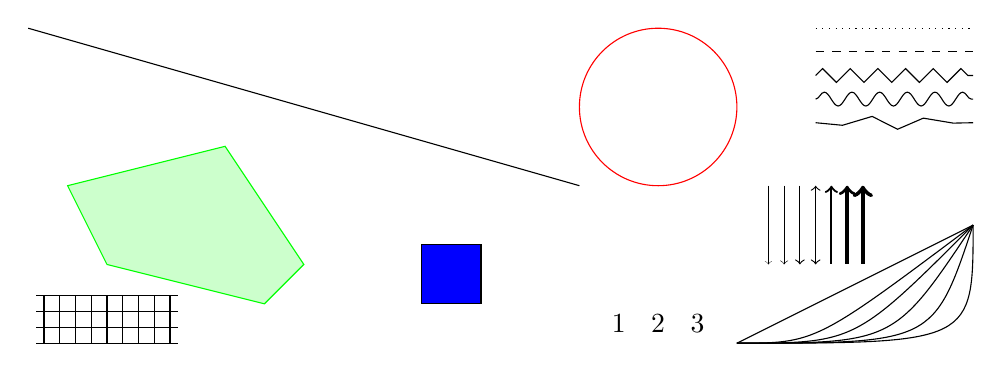
\begin{tikzpicture}[scale=1]
\draw (0,4) -- (7,2);
\draw[red] (8,3) circle(1cm);
\draw[fill=blue] (5,0.5) rectangle (5.75,1.25);
\draw[green, fill=white!80!green] (1,1) -- (3,0.5) -- (3.5,1) -- (2.5,2.5) -- (0.5,2) -- (1,1);
\draw[->, ultra thin] (9.4,2) -- (9.4,1);
\draw[->, very thin] (9.6,2) -- (9.6,1);
\draw[->, thin] (9.8,2) -- (9.8,1);
\draw[<->] (10,2) -- (10,1);
\draw[<-, thick] (10.2,2) -- (10.2,1);
\draw[<-, very thick] (10.4,2) -- (10.4,1);
\draw[<-, ultra thick] (10.6,2) -- (10.6,1);
\draw (7.5,0.25) node{1};
\draw (8,0.25) node{2};
\draw (8.5,0.25) node{3};
\draw[dotted] (10,4) -- (12,4);
\draw[dashed] (10,3.7) -- (12,3.7);
\draw[decorate, decoration=zigzag] (10,3.4) -- (12,3.4);
\draw[decorate, decoration=snake] (10,3.1) -- (12,3.1);
\draw[decorate, decoration=random steps] (10,2.8) -- (12,2.8);
\draw (9,0) -- (12,1.5);
\draw (9,0) .. controls (10,0) .. (12,1.5);
\draw (9,0) .. controls (10.5,0) .. (12,1.5);
\draw (9,0) .. controls (11,0) .. (12,1.5);
\draw (9,0) .. controls (11.5,0) .. (12,1.5);
\draw (9,0) .. controls (12,0) .. (12,1.5);
\draw[step=.2](0.1,0) grid (1.9,.6);
\end{tikzpicture}
\end{center}
\end{figure}

What the commands are doing: \\

\begin{compactitem}
\item \verb+[scale=1]+: Scales the figure with the dimensions given (in centimeters).  Increase (or decrease) the scale to expand (or shrink) the figure.
\item \verb+\draw (0,4) -- (7,2);+: Draws a straight line between coordinate points (2,3) and (7,2)..
\item \verb+\draw[red] (8,3) circle(1cm);+: Draws a circle colored red, centered at (8,3) and with radius of 1 centimeter.
\item \verb+\draw[fill=blue] (5,0.5) rectangle (5.75,1.25);+: Draws a rectangle (in this case a square) defined by corners at (5,0.5) and (5.75,1.25), and fills it blue.
\item \verb+\draw[green, fill=white!80!green] (1,1) -- (3,0.5) ... (0.5,2) -- (1,1);+: Draws a polygon region defined by the coordinates given, colored green and shaded a lighter green (80\% white, 20\% green).
\item \verb+\draw[->, ultra thin]...+: Draws a series of lines of varying thicknesses with arrows on one or both ends.
\item \verb+\draw (7.5,0.25) node{1};+: Draws a node with text `1' at coordinate point (7.5,0.25)
\item \verb+\draw[dotted]+: Draws a dotted (or dashed) line.
\item \verb+\draw[decorate,decoration=zigzag]+: Draws an object where the lines are `decorated' or modified in some way (zigzag, snake, bumpy, random steps, text, a series of various symbols, etc).
\item \verb+\draw (9,0) .. controls (12,0) .. (12,15);+: Draws a curved line going from (9,0) to (12,1.5) with a `control point' at (12,0) that pulls it into a bend.  The line starts out toward the control point, then curves to the end point.
\item \verb+\draw[step=.2](0.1,0) grid (1.9,.6);+: Draws a grid with the specified step width covering the specified area.  Note that if you want the grid closed (like the top and bottom) you should include limits divisible by the step width, and if you want the grid open (like the left and right) you should include limits which are not.\\
\end{compactitem}

\clearpage

This can be used to create a one-dimensional spatial model with some key points highlighted and labeled:\\

\begin{figure}[h!]
\begin{center}
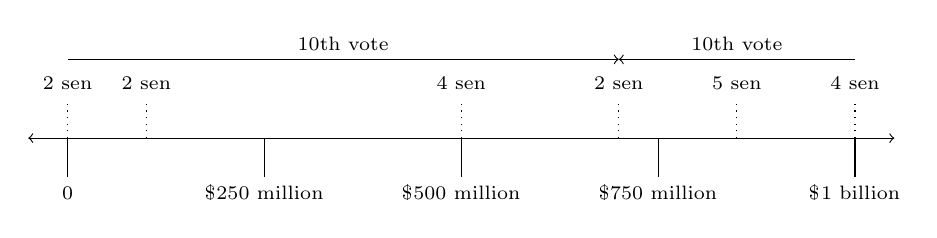
\begin{tikzpicture}[scale=1]
\draw[<->] (-.5,0) -- (10.5,0);
\draw (0,0) -- (0,-.5);
\draw (0,-.7) node{\scriptsize{0}};
\draw (2.5,0) -- (2.5,-.5);
\draw (2.5,-.7) node{\scriptsize{\$250 million}};
\draw (5,0) -- (5,-.5);
\draw (5,-.7) node{\scriptsize{\$500 million}};
\draw (7.5,0) -- (7.5,-.5);
\draw (7.5,-.7) node{\scriptsize{\$750 million}};
\draw (10,0) -- (10,-.5);
\draw (10,-.7) node{\scriptsize{\$1 billion}};
\draw (0,.7) node{\scriptsize{2 sen}};
\draw[dotted] (0,0) -- (0,.5);
\draw (1,.7) node{\scriptsize{2 sen}};
\draw[dotted] (1,0) -- (1,.5);
\draw (5,.7) node{\scriptsize{4 sen}};
\draw[dotted] (5,0) -- (5,.5);
\draw (7,.7) node{\scriptsize{2 sen}};
\draw[dotted] (7,0) -- (7,.5);
\draw (8.5,.7) node{\scriptsize{5 sen}};
\draw[dotted] (8.5,0) -- (8.5,.5);
\draw (10,.7) node{\scriptsize{4 sen}};
\draw[dotted] (10,0) -- (10,.5);
\draw[->] (0,1) -- (7,1);
\draw (3.5,1.2) node{\scriptsize{10th vote}};
\draw[<-] (7,1) -- (10,1);
\draw (8.5,1.2) node{\scriptsize{10th vote}};
\end{tikzpicture}
\end{center}
\end{figure}

\vspace{1cm}

You can extend this, along with many additional features, to draw anything else you need.  It works quite well for anything you'd like to show on a coordinate axis, such as two-dimensional spatial models or patterns over time, as well as any other drawings or flow charts you need..\\

\begin{figure}[h!]
\begin{center}
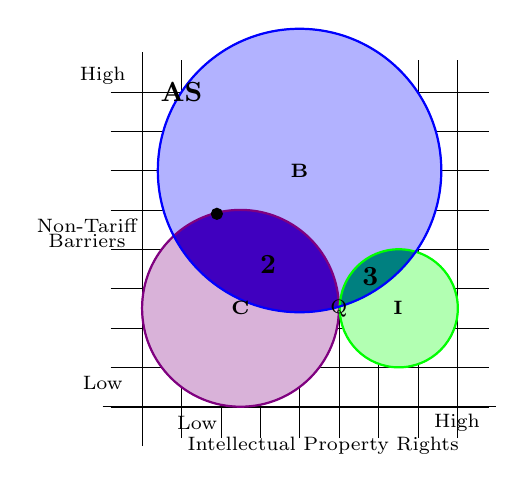
\begin{tikzpicture}[scale=1]
\draw[step=.5,black, ultra thin](-.4,-.4) grid (4.4,4.4);
\draw (-.5,0) -- (4.5,0);
\draw (-.7, 2.3) node{\scriptsize{Non-Tariff}};
\draw (-.7, 2.1) node{\scriptsize{Barriers}};
\draw (-.5, 4.2) node{\scriptsize{High}};
\draw (-.5, 0.3) node{\scriptsize{Low}};
\draw (0,-.5) -- (0,4.5);
\draw (2.3, -.5) node{\scriptsize{Intellectual Property Rights}};
\draw (4, -.2) node{\scriptsize{High}};
\draw (.7, -.2) node{\scriptsize{Low}};
\def\chinacircle{(1.25,1.25) circle(1.25cm)};
\def\indiacircle{(3.26,1.25) circle(0.75cm)};
\def\brazilcircle{(2,3) circle(1.8cm)};
\filldraw[fill=white!70!violet] \chinacircle;
\filldraw[fill=white!70!green] \indiacircle;
\filldraw[fill=white!70!blue] \brazilcircle;
\begin{scope}
    \clip \brazilcircle;
    \fill[green!50!blue] \indiacircle;
\end{scope}
\begin{scope}
    \clip \brazilcircle;
    \fill[violet!50!blue] \chinacircle;
\end{scope}
\draw[violet, thick] \chinacircle;
\draw[green, thick] \indiacircle;
\draw[blue, thick] \brazilcircle;
\draw (2.5,1.25) node{\scriptsize{Q}};
\draw (1.25,1.25) node{\scriptsize{\textbf{C}}};
\draw (3.25,1.25) node{\scriptsize{\textbf{I}}};
\draw (2,3) node{\scriptsize{\textbf{B}}};
\draw (1.6, 1.8) node{\textbf{2}};
\draw (2.9, 1.65) node{\textbf{3}};
\draw (.5, 4) node{\textbf{AS}};
\filldraw[fill=black] (.95,2.45) circle(2pt);
\end{tikzpicture}
\hspace{.5cm}
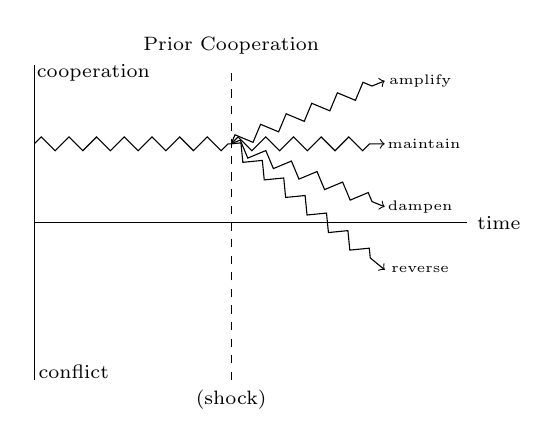
\begin{tikzpicture}[scale=1]
\draw (0,0) -- (5.5,0);
\draw (5.9,0) node{\scriptsize{time}};
\draw[dashed] (2.5,-2) -- (2.5,2);
\draw (2.5,-2.25) node{\scriptsize{(shock)}};
\draw (0,-2) -- (0,2);
\draw (.75,1.9) node{\scriptsize{cooperation}};
\draw (.5,-1.9) node{\scriptsize{conflict}};
\draw (2.5, 2.25) node{\scriptsize{Prior Cooperation}};
\draw[decorate,decoration=zigzag] (0,1.0) -- (2.5,1);
\draw[->, decorate,decoration={zigzag, post length=3}] (2.5,1) -- (4.45,1.8);
\draw[->, decorate,decoration={zigzag, post length=3}] (2.5,1) -- (4.45,1.0);
\draw[->, decorate,decoration={zigzag, post length=3}] (2.5,1) -- (4.45,.2);
\draw[->, decorate,decoration={zigzag, post length=3}] (2.5,1) -- (4.45,-.6);
\draw (4.9,1.8) node{\tiny{amplify}};
\draw (4.95,1.0) node{\tiny{maintain}};
\draw (4.9,.2) node{\tiny{dampen}};
\draw (4.9,-.6) node{\tiny{reverse}};
\end{tikzpicture}
\\ \vspace{.6cm}
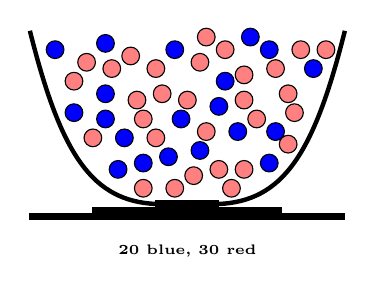
\begin{tikzpicture}[scale=.8]
\filldraw (-2.5,0) rectangle(2.5,.1);
\filldraw (-1.5,.1) rectangle (1.5,.2);
\filldraw (-.5,.2) rectangle (.5,.3);
\draw[ultra thick] (.5,.25) .. controls (1.5,.3) and (2,1) .. (2.5,3);
\draw[ultra thick] (-.5,.25) .. controls (-1.5,.3) and (-2,1) .. (-2.5,3);
\filldraw[fill=white!50!red] (-1.8,2.2) circle (4pt);
\filldraw[fill=white!50!red] (-1.6,2.5) circle (4pt);
\filldraw[fill=white!50!red] (-1.5,1.3) circle (4pt);
\filldraw[fill=white!50!red] (-.9,2.6) circle (4pt);
\filldraw[fill=white!50!red] (-.8,1.9) circle (4pt);
\filldraw[fill=white!50!red] (-.7,.5) circle (4pt);
\filldraw[fill=white!50!red] (-.5,1.3) circle (4pt);
\filldraw[fill=white!50!red] (-.7,1.6) circle (4pt);
\filldraw[fill=white!50!red] (-.5,2.4) circle (4pt);
\filldraw[fill=white!50!red] (-.2,.5) circle (4pt);
\filldraw[fill=white!50!red] (0,1.9) circle (4pt);
\filldraw[fill=white!50!red] (.2,2.5) circle (4pt);
\filldraw[fill=white!50!red] (.3,1.4) circle (4pt);
\filldraw[fill=white!50!red] (.6,2.7) circle (4pt);
\filldraw[fill=white!50!red] (.7,.5) circle (4pt);
\filldraw[fill=white!50!red] (.9,.8) circle (4pt);
\filldraw[fill=white!50!red] (.9,1.9) circle (4pt);
\filldraw[fill=white!50!red] (.9,2.3) circle (4pt);
\filldraw[fill=white!50!red] (1.1,1.6) circle (4pt);
\filldraw[fill=white!50!red] (1.4,2.4) circle (4pt);
\filldraw[fill=white!50!red] (1.6,1.2) circle (4pt);
\filldraw[fill=white!50!red] (1.6,2.0) circle (4pt);
\filldraw[fill=white!50!red] (1.7,1.7) circle (4pt);
\filldraw[fill=white!50!red] (1.8,2.7) circle (4pt);
\filldraw[fill=white!50!red] (2.2,2.7) circle (4pt);
\filldraw[fill=blue] (-2.1,2.7) circle (4pt);
\filldraw[fill=blue] (-1.8,1.7) circle (4pt);
\filldraw[fill=blue] (-1.3,1.6) circle (4pt);
\filldraw[fill=blue] (-1.3,2.0) circle (4pt);
\filldraw[fill=blue] (-1.3,2.8) circle (4pt);
\filldraw[fill=white!50!red] (-1.2,2.4) circle (4pt);
\filldraw[fill=blue] (-1.1,.8) circle (4pt);
\filldraw[fill=blue] (-1.0,1.3) circle (4pt);
\filldraw[fill=blue] (-.7,.9) circle (4pt);
\filldraw[fill=white!50!red] (-.4,2.0) circle (4pt);
\filldraw[fill=blue] (-.3,1.0) circle (4pt);
\filldraw[fill=blue] (-.2,2.7) circle (4pt);
\filldraw[fill=blue] (-.1,1.6) circle (4pt);
\filldraw[fill=white!50!red] (.1,.7) circle (4pt);
\filldraw[fill=blue] (.2,1.1) circle (4pt);
\filldraw[fill=white!50!red] (.3,2.9) circle (4pt);
\filldraw[fill=white!50!red] (.5,.8) circle (4pt);
\filldraw[fill=blue] (.5,1.8) circle (4pt);
\filldraw[fill=blue] (.6,2.2) circle (4pt);
\filldraw[fill=blue] (.8,1.4) circle (4pt);
\filldraw[fill=blue] (1.0,2.9) circle (4pt);
\filldraw[fill=blue] (1.3,.9) circle (4pt);
\filldraw[fill=blue] (1.3,2.7) circle (4pt);
\filldraw[fill=blue] (1.4,1.4) circle (4pt);
\filldraw[fill=blue] (2.0,2.4) circle (4pt);
\draw (0,-.5) node{\tiny{\textbf{20 blue, 30 red}}};
\end{tikzpicture}
\end{center}
\end{figure}


A few additional commands introduced here that are useful for diagrams with shapes that interact with each other: \\

\begin{compactitem}
\item \verb+\def\chinacircle{(1.25,1.25) circle(1.25cm)};+: `Defines' an object and names it without drawing it (yet), so you can use it in other operations and commands.
\item \verb+\filldraw[...]...+: Draws an object and fills it in at the same time, subject to commands specified in the rest of the command (or wherever the object is defined).  Note that the package draws each subsequent object on top of everything before it, so if you have two objects in the same space (e.g. a circle that is shaded in with the a label in the middle) make sure you order the draw commands such that objects on top come later.
\item \verb+\begin{scope} ... \end{scope}+: Defines the `scope' of an area for a fill command as the space where the `brazilcircle' and `indiacircle' objects overlap.\\
\end{compactitem}

\clearpage

\section{Quick and Dirty Freehand}

Finally, if you want a diagram but don't feel like wading through the coding, a quick and dirty way to do it is using a free program TeXCAD that handles these moderately well.  It works somewhat like MS Paint but much crisper, includes a few handy features for technical drawings, and it plays well with \LaTeX.  It will produce a file that you can put directly into your document using \verb+input filename.pic+ or it will give you code that will produce your picture, which you can then edit as needed.  Just to get a sense of what it can do:

\begin{center}
%\input texcadsample.pic
\begin{scriptsize}
(un-comment the picture command to display the picture if you have the file)
\end{scriptsize}
\end{center}


% NOTE: If this file is failing to compile, check if you're missing this file from the directory.  If that's the issue, either get the picture or comment-out the bit of code above.



\section{References}

The .sgamevar and .egameps packages were written by Martin Osborne, an economist at the University of Toronto, so the best resource for them is his website: \href{http://www.economics.utoronto.ca/osborne/latex/}{http://www.economics.utoronto.ca/osborne/latex/}.  The sgame.pdf and egame.pdf guide documents are particularly useful, both for debugging and for discovering more advanced features of the packages. \\

The .tikz and .pgf packages were designed by Till Tantau, a computer scientist at the University of L\"{u}beck.  The best resource for learning how it works is his extensive online manual, available at \href{http://www.ctan.org/tex-archive/graphics/pgf/base/doc/generic/pgf/pgfmanual.pdf}{http://www.ctan.org/tex-archive/graphics/pgf/base/doc/generic/pgf/pgfmanual.pdf}.  It is 560 pages long, but fortunately has a table of contents and an index and is searchable.  Most of the information you might want about how to do various things is in the `I. Tutorials and Guidelines' section, which is very user-friendly (and surprisingly funny).  There are also examples of code for all sorts of fun stuff in tikz at \href{www.texample.net}{www.texample.net}. \\

TeXCad is available for free download at \href{http://texcad.sourceforge.net/}{http://texcad.sourceforge.net/}.\\

